\documentclass[conference]{IEEEtran}

\usepackage{cite}
\usepackage{pgfplots}
\usepackage{url}
\pgfplotsset{compat=1.18}

\title{Reproducing Ascon v1.2 Software Performance:\\
An Evaluation of Message Size and Implementation Choices}

\author{\IEEEauthorblockN{Author name}
\IEEEauthorblockA{Institution\\
Email address}}

\begin{document}
\maketitle

\begin{abstract}
This paper partially reproduces the software performance evaluation of
Ascon v1.2 and examines message size, associated data, implementation, and
compiler optimization. We tested reference and optimized implementations of
Ascon-128 and Ascon-128a on one Windows workstation, including differential
checks against a separately developed implementation. In the optimized
implementation at 1536 bytes, the median elapsed times were 5.828 and
3.835 microseconds, respectively. Their ratio was 1.52, compared with a
reported cycles-per-byte ratio of 1.49 for a different processor in the
original paper. Timer, hardware, software, and statistic differences preclude
an absolute performance comparison. Short-message, associated-data, and
compiler-setting results illustrate workload and implementation sensitivity.
The measurements are exploratory and do not establish security or performance
on constrained devices.
\end{abstract}

\begin{IEEEkeywords}
Ascon, authenticated encryption, reproducibility, software performance,
lightweight cryptography
\end{IEEEkeywords}

\section{Introduction}
Lightweight cryptography aims to provide cryptographic primitives suitable for
constrained systems. Dobraunig \emph{et al.} present the Ascon v1.2 family and
report software performance for multiple processors and message
lengths~\cite{ascon2021}. Reproducing those results requires more than running
the authors' software: the algorithm version, workload, implementation,
compiler, timing method, and hardware must also be identified.

This study asks: \emph{How do message size, associated-data length,
implementation choice, and compiler settings affect the software performance
of Ascon-128 and Ascon-128a, and how do the measured trends compare with the
2021 paper?} The primary experiment reconstructs the empty-associated-data
workload in Table~19 of the original paper. Further experiments investigate
block-boundary behavior and implementation sensitivity. This is a partial
reproduction focused on software; it does not reproduce the original hardware,
energy, area, or security evaluations.

\section{Background and Original Research}
Ascon-128 and Ascon-128a are authenticated-encryption schemes with associated
data (AEAD). Both use a 128-bit key, nonce, and authentication tag.
Ascon-128 processes data in 8-byte blocks and uses six rounds for the
intermediate permutation; Ascon-128a uses 16-byte blocks and eight intermediate
rounds. Both use 12 rounds for initialization and finalization~\cite{ascon2021}.
These design choices motivate measuring short inputs and block boundaries
separately from long-message throughput.

Table~19 in the original paper reports encryption performance in cycles per
byte for empty associated data, across different processors and plaintext
lengths~\cite{ascon2021}. For example, on an Intel Core i5-6300U, the reported
values for a 1536-byte message are 11.9 cycles per byte for Ascon-128 and
8.0 for Ascon-128a. These values are a published reference, not measurements
of the computer used in this study.

The later NIST standard specifies Ascon-AEAD128 and other primitives; its
specification must not be substituted for Ascon v1.2 in a historical
reproduction~\cite{nist2025}. The upstream repository identifies changes in
byte order and initialization values between the submission and the
standardized algorithms~\cite{asconstandardrepo}.

\subsection{Expected Performance Trade-offs}
Both AEAD variants must initialize a state, process the input, and finalize a
tag, even when the plaintext is short. Therefore, a per-byte metric may be
dominated by fixed work for small inputs. At larger sizes, the amount of data
processed per intermediate permutation becomes more important. Ascon-128a
has twice the data rate of Ascon-128 but a larger intermediate-round count;
the effect on an actual processor also depends on generated machine code and
memory operations. A rate comparison alone does not determine the observed
performance of either implementation.

Associated data is authenticated even though it is not included in the
ciphertext length. Reporting only plaintext bytes in the denominator can
therefore obscure substantial work when the associated data is nonempty.
This motivates comparing time per operation as well as time per byte, and
keeping the associated-data size visible in all extended workloads.

\section{Reproduction Methodology}
\subsection{Artifacts and Correctness}
The starting implementation is the upstream \texttt{v1.2.8} release at commit
\texttt{b359dc54e323}~\cite{asconrepo}.
This release is later than the 2021 paper, so it must not be assumed to be the
exact benchmark artifact used by the authors.

The initial configuration builds the reference (\texttt{ref}) and optimized
64-bit (\texttt{opt64}) implementations of both AEAD variants. It also builds
Ascon-Hash for correctness testing. Each Release configuration passed six
repository known-answer tests. For each of the four AEAD combinations, our
additional check covered 130 plaintext/associated-data length pairs from 0 to
256 bytes, successful decryption, and rejection of altered ciphertext, tags,
associated data, nonces, and a ciphertext shorter than the tag.

The additional check compares encryption and decryption with the separately
developed lightweight-crypto implementation at a pinned commit~\cite{lightweightcrypto}.
All four differential checks passed. Its externally hosted KAT files match the
repository vectors after newline normalization, so the two copies are not
counted as independent vector evidence. The checks increase confidence in
functional compatibility for the tested cases; they do not prove security or
correctness for all possible inputs.

\subsection{Experimental Questions and Workloads}
The experiments were:
\begin{enumerate}
  \item \textbf{Published-workload reconstruction:} encrypt messages of 1, 8,
  16, 32, 64, and 1536 bytes with zero bytes of associated data. Report both
  variants and compare trends with Table~19. The paper's ``Long'' entry is
  not assigned a measured length here; an additional 4096-byte case is a
  separately labeled extension, not an exact reproduction of that column.
  \item \textbf{Block-boundary analysis:} additionally measure plaintext
  lengths 0, 7, 9, 15, 17, 31, and 33 bytes. Test whether runtime changes near
  8- and 16-byte boundaries, and discuss the role of padding and permutation
  calls. Treat the observed pattern as an empirical question.
  \item \textbf{Associated-data sensitivity:} for plaintext lengths 1, 16,
  64, and 1536 bytes, measure associated-data lengths 0, 1, 8, 16, 32, and
  256 bytes. This is an extension to Table~19, not a reconstruction of its
  empty-associated-data workload.
  \item \textbf{Implementation and compiler sensitivity:} compare
  \texttt{ref} and \texttt{opt64} using identical inputs and compiler settings.
  Repeat selected   sizes with MSVC speed- and size-optimization settings in separate build
  directories. The two Release configurations use \texttt{/O2} and
  \texttt{/O1}, respectively, with \texttt{/MD}, \texttt{/Ob2}, and
  \texttt{/DNDEBUG}; compiler command records are archived.
\end{enumerate}

These experiments measure encryption, including tag generation; they do not
include file I/O or memory allocation in the timed region. Key, nonce,
plaintext, and associated data are prepared beforehand. Benchmark-only inputs
must be clearly labeled: real deployments must not reuse a nonce with the
same key.

\subsection{Measurement Procedure}
The host was an Intel Core i5-12400 with Windows 11 Home 64-bit, MSVC
19.51.36256, and CMake 4.4.4. Windows used its Balanced power plan; background
load was not measured and the machine was not exclusively reserved. Each
benchmark thread was pinned to the lowest processor in its allowed affinity
mask, which was logical processor 0 for these runs. CPU frequency and boosting
were not locked. The same deterministic input buffers were reused across
operations; this measures a warm-buffer workload rather than file or network
performance.

After 32 warm-up calls per case, the harness doubled the batch size until the
shortest of three trial batches reached 2 ms. It then measured 30 batches for
each case in each of three repeated program invocations. The complete matrix
contains 24,480 batches across 272 configurations. Configurations were run in
a fixed order, not randomized. The raw counter ticks, batch sizes, affinity
mask, timer frequency, build flags, source hashes, and environment are
archived with the study.

The reported time per operation is elapsed counter time divided by the number
of encryptions in a batch. We summarize the 90 batches per configuration by
their pooled median and interquartile range (IQR), and also retain the three
run medians. These are descriptive statistics: batches from the same
invocation are not independent experiments, and the IQR is not a confidence
interval. Time per plaintext byte is undefined for the zero-length case.

The timer is Windows \texttt{QueryPerformanceCounter}, with a reported
frequency of 10 MHz. It measures elapsed time, including preemption, not core
cycles. The harness also records adjacent timer reads; their median difference
was zero ticks and their 99th percentile was one tick, subject to timer
resolution and scheduling. That measurement is not subtracted. Of the 24,480
batches, 767 lasted less than 2 ms despite calibration; observed durations
ranged from 1.252 to 104.321 ms. No batches were removed. The long tail and
sub-threshold batches show that calibration and affinity did not eliminate
noise.

The repository's separate \texttt{getcycles} tool uses an unserialized
\texttt{RDTSC} counter on x86. Its output is not assumed to be actual core
cycles. Neither TSC ticks nor our elapsed-time values are interchangeable with
the original table's cycles per byte.

\section{Results}
\subsection{Comparison with Published Work}
Table~\ref{tab:comparison} places the published values alongside our local
measurements, but the columns have different units, hardware, and measurement
procedures. For 1536 bytes the published Ascon-128/Ascon-128a ratio is
$11.9/8.0 = 1.49$; our corresponding \texttt{opt64} median-time ratio is
$5827.8/3835.3 = 1.52$. Both favor Ascon-128a for this long input, but their
numerical closeness does not establish an exact reproduction. Our 4096-byte
ratio was 1.60; this is an extension and is not the paper's unspecified
``Long'' input.

\begin{table}[htbp]
\caption{Published i5-6300U values versus local i5-12400 \texttt{opt64}
\texttt{/O2} medians with empty associated data. Units and platforms differ.}
\label{tab:comparison}
\centering
\begin{tabular}{rcccc}
\hline
Bytes & \multicolumn{2}{c}{Paper: cycles/byte} &
        \multicolumn{2}{c}{Local: ns/op} \\
& 128 & 128a & 128 & 128a \\
\hline
1    & 367  & 365  & 138.2  & 141.3 \\
8    & 58   & 47   & 159.4  & 134.6 \\
16   & 35   & 31   & 192.4  & 183.8 \\
32   & 23   & 19   & 259.6  & 221.9 \\
64   & 17.6 & 13.5 & 371.0  & 291.5 \\
1536 & 11.9 & 8.0  & 5827.8 & 3835.3 \\
\hline
\end{tabular}

\smallskip
\footnotesize Published values are from Table~19 of~\cite{ascon2021}.
Local results are pooled medians of 90 batches per row.
\end{table}

Fig.~\ref{fig:length} shows the measured progression across all nonempty
plaintext lengths for the same configuration. Both axes are logarithmic; the
zero-length case is excluded because it cannot be placed on a logarithmic
axis.

\begin{figure}[htbp]
\centering
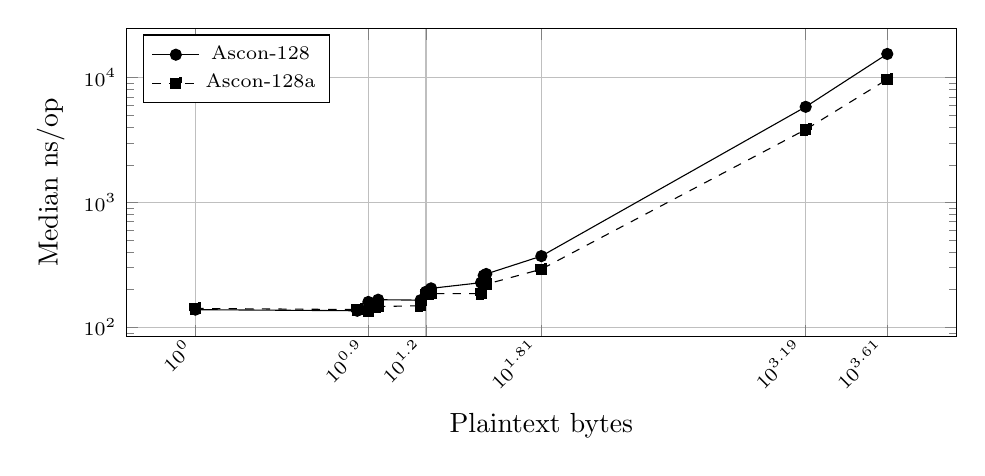
\begin{tikzpicture}
\begin{loglogaxis}[
  width=\columnwidth, height=5.5cm,
  xlabel={Plaintext bytes}, ylabel={Median ns/op},
  xtick={1,8,16,64,1536,4096},
  xticklabel style={font=\scriptsize, rotate=45, anchor=east},
  yticklabel style={font=\scriptsize},
  legend style={font=\scriptsize, at={(0.02,0.98)}, anchor=north west},
  grid=major]
\addplot[black, solid, mark=*] coordinates {
  (1,138.196) (7,135.408) (8,159.390) (9,166.034)
  (15,164.670) (16,192.419) (17,204.703) (31,227.335)
  (32,259.570) (33,266.888) (64,370.978) (1536,5827.832)
  (4096,15459.766)};
\addlegendentry{Ascon-128}
\addplot[black, dashed, mark=square*] coordinates {
  (1,141.266) (7,138.397) (8,134.641) (9,146.280)
  (15,148.630) (16,183.841) (17,185.980) (31,185.916)
  (32,221.924) (33,220.807) (64,291.473) (1536,3835.254)
  (4096,9679.883)};
\addlegendentry{Ascon-128a}
\end{loglogaxis}
\end{tikzpicture}
\caption{Pooled median time per encryption for \texttt{opt64} \texttt{/O2}
with empty associated data. Variability for selected cases appears in the
tables.}
\label{fig:length}
\end{figure}

\subsection{Short Messages and Associated Data}
Table~\ref{tab:boundary} shows selected pooled medians and IQRs around block
boundaries. For Ascon-128, the median rose from 135.4 ns at seven bytes to
159.4 ns at eight; Ascon-128a's corresponding medians were 138.4 and 134.6 ns.
At 15 and 16 bytes, Ascon-128a's medians were 148.6 and 183.8 ns. The
pattern is consistent with the differing block rates, but the measured
distributions overlap and the cases were not randomized. These observations
should be repeated under lower noise before drawing strong conclusions about
individual-byte differences.

\begin{table}[htbp]
\caption{Short-message medians [IQR], in ns/op, \texttt{opt64} \texttt{/O2},
zero associated data.}
\label{tab:boundary}
\centering
\begin{tabular}{rcc}
\hline
Bytes & Ascon-128 & Ascon-128a \\
\hline
7  & 135.4 [129.2, 148.3] & 138.4 [128.6, 153.8] \\
8  & 159.4 [151.2, 177.0] & 134.6 [125.9, 152.9] \\
15 & 164.7 [157.2, 179.0] & 148.6 [135.3, 168.0] \\
16 & 192.4 [183.5, 214.6] & 183.8 [168.0, 204.7] \\
\hline
\end{tabular}
\end{table}

Table~\ref{tab:ad} extends the workload to nonempty associated data for a
16-byte plaintext. The 256-byte associated-data case had considerably higher
median time than the empty case for both variants. The one-byte and eight-byte
Ascon-128a results do not increase monotonically; their IQRs overlap, so the
results should not be read as evidence that processing more associated data
is intrinsically faster. They demonstrate that empty-associated-data
benchmarks omit a potentially important application cost.

\begin{table}[htbp]
\caption{Associated-data experiment: 16-byte plaintext, \texttt{opt64}
\texttt{/O2}. Values are median [IQR] ns/op.}
\label{tab:ad}
\centering
\begin{tabular}{rcc}
\hline
AD bytes & Ascon-128 & Ascon-128a \\
\hline
0   & 192.4 [183.5, 214.6] & 183.8 [168.0, 204.7] \\
1   & 230.6 [220.2, 257.3] & 220.1 [208.5, 239.7] \\
8   & 253.1 [240.6, 273.3] & 211.4 [202.0, 224.3] \\
16  & 279.8 [265.8, 309.1] & 256.5 [244.0, 290.8] \\
256 & 1189.6 [1119.3, 1350.5] & 834.2 [801.8, 931.3] \\
\hline
\end{tabular}
\end{table}

\subsection{Implementation and Compiler Sensitivity}
Table~\ref{tab:flags} compares all four AEAD implementations at 1536 bytes.
For the reference implementation, the \texttt{/O1} pooled medians were about
1.23 and 1.34 times the \texttt{/O2} medians for Ascon-128 and Ascon-128a,
respectively. In the Ascon-128 \texttt{/O2} case, the reference median was
lower than the \texttt{opt64} median, despite the latter's name. Their IQRs
overlap; this observation does not establish a general ranking. A compiler
setting or implementation label alone is insufficient to predict performance
across workloads and machines.

\begin{table}[htbp]
\caption{1536-byte plaintext, empty AD. Median [IQR] ns/op over 90 batches.}
\label{tab:flags}
\centering
\begin{tabular}{llr}
\hline
Variant & Implementation / flag & Time in ns/op \\
\hline
128  & ref /O2   & 5517.1 [5223.4, 6000.7] \\
128  & opt64 /O2 & 5827.8 [5641.1, 6442.5] \\
128  & ref /O1   & 6757.0 [6343.5, 7691.9] \\
128  & opt64 /O1 & 6194.9 [5870.4, 7002.8] \\
128a & ref /O2   & 3907.8 [3704.1, 4451.2] \\
128a & opt64 /O2 & 3835.3 [3661.9, 4262.2] \\
128a & ref /O1   & 5248.3 [5008.5, 6004.4] \\
128a & opt64 /O1 & 4255.2 [4021.4, 4472.6] \\
\hline
\end{tabular}
\end{table}

\section{Discussion and Reproducibility Assessment}
The strongest supported comparison is directional: on this host and selected
implementation, Ascon-128a had lower median elapsed time than Ascon-128 for
the 1536-byte workload, as in the original paper's i5-6300U row. The original
table reports cycles per plaintext byte, while our timer reports elapsed
time. Consequently, the raw values cannot be converted into a meaningful
speedup between machines without further measurement and assumptions.
Moreover, the selected \texttt{v1.2.8} source postdates publication; the
original compiler configuration, exact source revision and aggregation
method require further artifact investigation.

The fixed execution order can confound differences between settings with
changes in system load or frequency. The run medians and pooled IQRs expose
some variability but do not eliminate it. The original hardware was not
available, and this work did not reproduce other CPU families or embedded
platforms. The paper's ``Long'' length remains unspecified in this
reconstruction. The 4096-byte extension is reported separately.

A first pilot used a single calibration trial and produced batches as short
as 0.0285 ms after a slow calibration sample. It is archived separately and
excluded from the results above. Using the shortest of three trial batches
reduced, but did not eliminate, short batches. This is a methodological
finding: even a plausible timer loop needs validation against its raw
durations, and calibration cannot substitute for an idle and controlled
environment.

The repository includes the test source, benchmark, scripts, raw batches,
summaries, environment information, independent-test report, and compiler
command records. Reproduction requires the stated Windows toolchain; the
separately licensed independent source must be obtained at its pinned
revision. MSVC also reported narrowing-conversion warnings in upstream
implementation files; the bounded test cases do not resolve correctness for
arbitrarily large inputs. The same test suite cannot establish constant-time behavior,
side-channel resistance, power consumption, or performance on a microcontroller.
Future work should use randomized case order, more independent sessions, a
quieter machine, and a validated core-cycle measurement to compare more
directly with the original experiments.

\section{Conclusion}
This study reconstructed selected Ascon v1.2 software workloads and found
the same long-message ordering between Ascon-128 and Ascon-128a as a published
example. Message size, associated data, implementation, and compiler settings
all affected the observed timings. Functional differential checks supported
the tested outputs, but the later source revision, different platform and
timer, and observed scheduling noise limit the strength of the reproduction.
The results should be treated as an exploratory partial reproduction rather
than a precise replication of the published cycle counts.

\bibliographystyle{IEEEtran}
\bibliography{references}

\end{document}
